\documentclass[a4paper]{article}
\usepackage[utf8]{inputenc}
\usepackage{multicol}
\usepackage{hyperref}
\usepackage[margin=1in]{geometry}
\usepackage{natbib}
\usepackage{graphicx}
\usepackage{enumerate}
\usepackage{float}
\usepackage{color}
\usepackage{caption}
\usepackage{wrapfig}
\usepackage{caption}
\usepackage{subcaption}
\restylefloat{table}

\title{Adjusting difficulty based on automatically generated models of player skill}
\author{Arjen Swellengrebel}
\date{\today}

\begin{document}

\maketitle

\begin{multicols*}{2}
\begin{abstract}
This is done using two subsystems, the first of which determines the level of emotional intensity of the player based on their behaviour in the game.
Secondly, a method for modelling the emotional reaction of a player to game situations is presented.
Finally, a practical example based on \emph{The Legend of Zelda} shows the accuracy of the results of this approach.
\end{abstract}

\section{Introduction}
To enhance the accessibility of a video game, and thereby increase its potential audience, it is advisable to present each player with an experience personalized to them \cite{playercentered}. Perhaps most notably, Valve's \emph{Left 4 Dead} uses a system called the "AI director" which changes the pacing of its combat sequences based on the performance of the players \cite{left4dead}. However, the AI director only removes threats when tension becomes too high.

The purpose of this thesis is to show how it is possible to modify much of the game's content to achieve a specific player experience. Rather than finding the optimal difficulty, the goal will be to find the effect each game element has on the experience.
\begin{itemize} \item[\textbf{1.}] How can the effect of game elements on the emotional intensity of its players be found? \end{itemize}
To answer this question, it is necessary to know the emotional reaction of a given player to a combination of game elements. Therefore, a secondary goal will be to estimate that reaction without pausing the game to ask the player.
\begin{itemize} \item[\textbf{2.}] How can the emotional state of a player be accurately determined using in-game data? \end{itemize}

To answer these questions, the proposed method has been applied to an example game based on \emph{The Legend of Zelda}. This environment is used to quantify the accuracy of this approach and demonstrates how it can be applied to players' different skill levels. It also shows how the system can be applied generically over different in-game settings, and provides an approach for predicting the effect of unseen elements.

\section{Related Work}
\textcolor{red}{write}

\section{Method}
The method proposed here consists of two subsystems. The first (hereafter the \emph{estimator}) estimates the amount of stress experienced after an encounter has been completed. This estimate is made using only information specific to the player's behaviour during that encounter. The estimator is constructed before runtime, using labeled data, and is applied equally to every player regardless of skill.

The second subsystem (hereafter the \emph{builder}) predicts the difficulty level of an encounter before it is presented to the player. By necessity, it uses only information which is set when the encounter starts. This model is constructed and updated at runtime, using the results of the estimator as a supervisory signal. The model is created individually for each player.

\subsection{Application}
\textcolor{red}{write}

\subsection{Data}
\textcolor{red}{improve}
The emotional intensity experienced by a player is measured on a scale from 1 to 10. Intensities of grade 1 through 5 are enjoyable difficulties. A difficulty of 1 means a complete absence of any difficulty, while 5 marks the maximum difficulty which is still enjoyable to the player. Grades of 6 through 10 represent inappropriate difficulties, 6 being just slightly too high, and 10 impossible to succeed at even with extensive practice.

Players were asked to play through a series of rooms containing variable numbers of enemies. In each of these rooms, three possible outcomes are possible: the player  defeats every enemy in the room, leaves the room prematurely, or loses all hearts and is defeated. In each of these cases the game was paused automatically and the player was asked to rate the perceived challenge of the room on the aforementioned scale. A description of the room was then recorded, along with a summary of the player's behaviour in that room and their report of its difficulty.

\subsection{Assumptions}
\textcolor{red}{improve}
The system relies on the assumption that the behaviour of a player experiencing some level of emotional intensity is the same regardless of skill. For example, a player who gets hit five times in a room will experience stress as a result of that fact, whether this is a skilled player fighting many enemies or a beginner fighting a single enemy. This assumption allows us to ascertain the stress level of a player without having to stop the game to ask them what it is.

As will be shown in section \ref{fig:results}, this assumption is robust enough to show reasonable accuracy in the data. By including a variable denoting the player's experience with video games, that section will attempt to show exactly how robust the assumption is.

\section{Implementation}
This project is based on the open-source video game \emph{Legend of Zelda: Mystery of Solarus DX} \cite{zeldasolarus}. Areas were randomly generated at runtime using Dormans and Bakkes' technique for generating missions and spaces \cite{missiongrammar}. For these experiments, however, areas were kept fairly linear so as to reduce time spent during user studies. 

\subsection{Game description}
The game area is divided into two sections, a forest and a dungeon. The forest is preceded by a tutorial section consisting of four rooms. The other two areas contain six rooms each. In the forest, players can freely move between areas at any time, while the dungeon has doors which only open when every enemy has been defeated. Additionally, dungeon rooms contain hazards which reduce the player's hit points on contact, while forest rooms do not.

The player starts the game with 24 hit points and a sword which does a single point of damage to every normal enemy. Throughout the experiment, the player can pick up two items that provide different ways of fighting enemies. The first is a glove which lets them pick up and throw rocks and bushes if available, both dealing two points of damage to enemies on a hit). The second is a bag of bombs which can be placed on the ground or thrown at enemies, also dealing two points of damage. 

Enemies are decided and placed each time the player enters a room. Normal rooms contain four possible types of enemies. These are the \emph{mandible}, a simple walking enemy, the \emph{minillosaur egg}, which remains stationary until the player approaches, the \emph{hardhat beetle} which pushes the player back when hit, and the \emph{knight soldier} which holds a sword which must be avoided. Every type of enemy must be hit three times to be defeated and deals two hit points of damage on a hit (equating half a heart). All types also have a small chance of giving the player a heart when they are defeated, which restores 4 hit points.

Two exceptions to this model are the tutorial room and the boss room. The tutorial rooms are simple forest locations which contain a single enemy each. The boss room is located at the end of the dungeon and contains a single \emph{papillosaur king}, a large enemy which shoots weaker versions of the \emph{minillosaur egg} enemy. This enemy must be defeated with three bombs, as it cannot be attacked with the sword.

\begin{figure*}
\centering
\begin{subfigure}[b]{0.45\textwidth}
  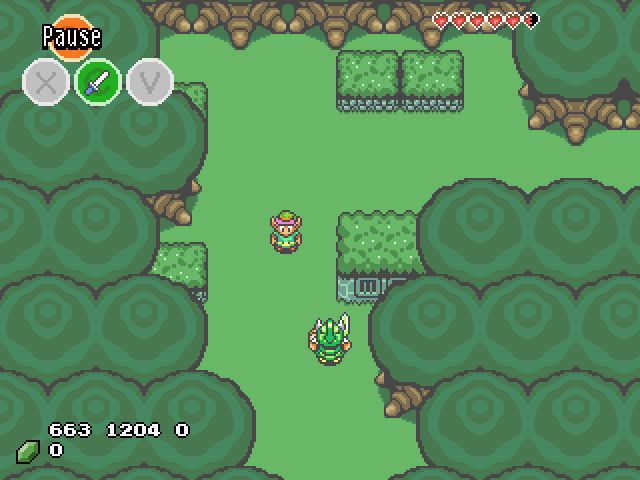
\includegraphics[width=\textwidth]{tutorialroom}
  \captionof{figure}{Tutorial room}
\end{subfigure} \hfill
\begin{subfigure}[b]{0.45\textwidth}
  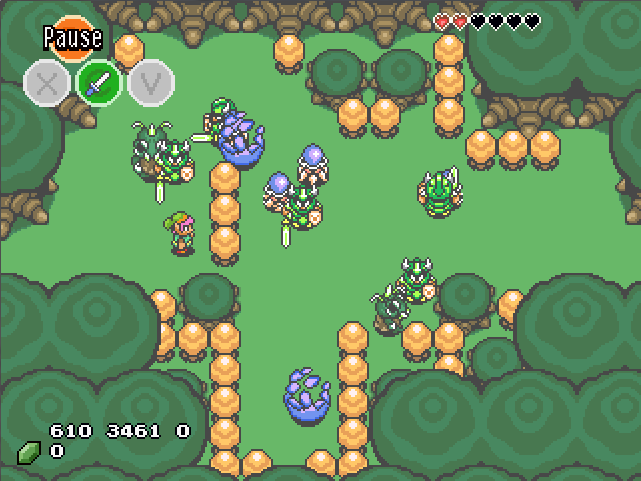
\includegraphics[width=\textwidth]{forestroom}
  \captionof{figure}{Example forest room}
\end{subfigure} \hfill
\begin{subfigure}[b]{0.45\textwidth}
  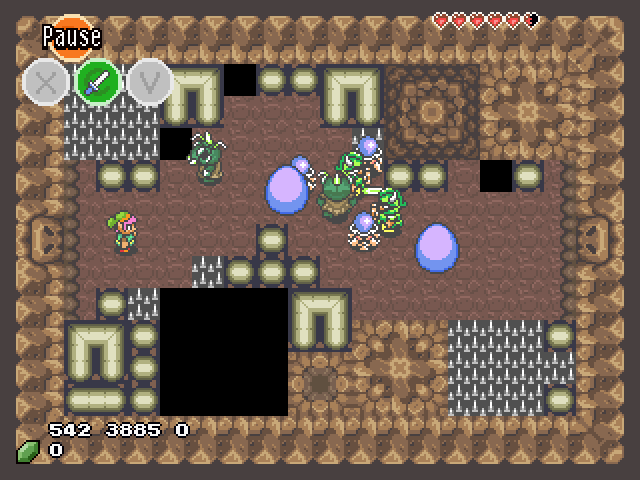
\includegraphics[width=\textwidth]{dungeonroom}
  \captionof{figure}{Example dungeon room}
\end{subfigure} \hfill
\begin{subfigure}[b]{0.45\textwidth}
  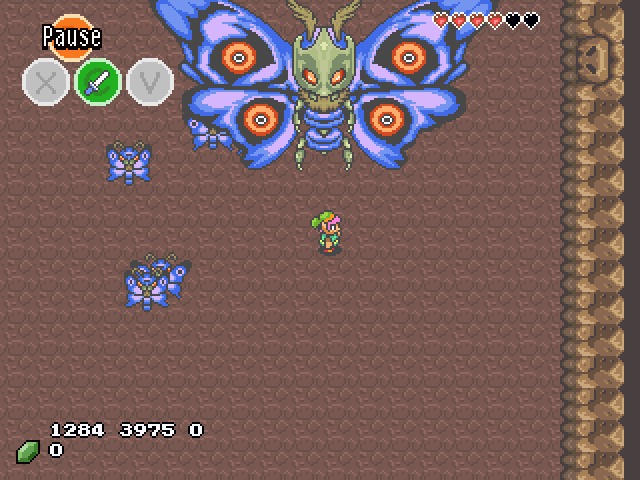
\includegraphics[width=\textwidth]{bossroom}
  \captionof{figure}{Final boss room}
\end{subfigure} \hfill
\end{figure*}

\subsection{Room construction}
\textcolor{red}{improve}
To gather the largest amount of data possible from each room, each player should be presented with challenges they can conceivably overcome. To do this, rooms were created based on informal data gathered early in the development of the project. While this method does not produce results representative of the final product, it does produce setups which will result in somewhat appropriate challenges while still varying the data. To create additional variety in the dataset, eight percent of all encounters were set to an extreme difficulty. In all other rooms, players were presented with intended difficulties of 2 through 6.

In order to start determining the right makeup of a combat encounter for a player, first gauge the reaction of that particular player to every possible enemy in the game must be estimated. Fortunately, this need coincides with the need to train the player in a reasonably safe environment. For these reasons, the player must first fight their way through a series of rooms that each contain one enemy, one room for each type. 

Once every enemy has been encountered once, enough data will be available to make a first estimate of the appropriate difficulty. Subsequent rooms will be constructed to slowly increase the difficulty for this player to a desirable level, starting at the lowest level. Starting at a lower difficulty decreases the risk of an encounter being constructed based on faulty data, which is a concern at this point because of sparsity. Each of the progressively more difficult rooms will increase the amount of data and thus decrease the margin of error on the formula. This way errors are most likely to occur in rooms with a low difficulty, which reduces the chance of an overshoot creating an impossible challenge for the player.

\section{Results} \label{fig:results}
Data was recorded from a total of 16 test subjects. In total, 302 encounters were recorded, each participant completing an average of 18.88 encounters with a standard deviation of 7.191. Five of the test subjects had no experience with action video games, six had some experience but no experience with the Legend of Zelda, and five had previous experience with the game. These groups account for 23.5\%, 43\% and 33\% of the data. Finally, 54\% of all recorded fights were inside the dungeon, and the final boss was seen eleven times in total. The intended difficulty of the encounters presented ranged from 1 to 7.558, with a 3.371 mean and 1.807 standard deviation.

\subsection{Models}
\textcolor{red}{complete}
The final model was generated using Weka \cite{weka}.

\textcolor{red}{prettify}
\begin{table*}[t]
\centering
\begin{tabular}{lcccc} \hline
Classifier & 
\begin{tabular}{c} Mean\\absolute\\error \end{tabular} & 
\begin{tabular}{c} Root\\mean\\squared\\error \end{tabular} & 
\begin{tabular}{c} Relative\\absolute\\error (\%) \end{tabular} & 
\begin{tabular}{c} Root\\relative\\squared\\error (\%) \end{tabular} \\
\hline
Pace regression & 1.1066 & 1.551 & 71.3851 & 82.9991 \\ \hline
SMO regression & 1.0634 & 1.6185 & 68.6005 & 86.6108 \\ \hline
M5 rules & 1.0933 & 1.4334 & 70.5283 & 76.7064 \\ \hline
Gaussian processes & 0.999 & 1.294 & 64.4455 & 69.2444 \\ \hline
\end{tabular}
\captionof{figure}{Accuracy of the builder}
\end{table*}

\subsection{Generalizability}
\textcolor{red}{write}

\section{Future Work}
\textcolor{red}{complete}
As written, the game places enemies in discrete encounters. Planning for emotional intensity will likely be more difficult when enemies are allowed to move into or out of the space the player is currently in. 

\section{Acknowledgements}
Much of the code for this project was provided by Norbert Heijne. His research concerning this engine can be found in an upcoming paper.

\bibliographystyle{plain}
\begin{thebibliography}{9}

\bibitem{playercentered}
D. Charles, M. McNeill, M. McAlister, M. Black, A. Moore, K. Stringer, J. Kucklich, and A. Kerr, 
\emph{Player-centered design: Player modeling and
adaptive digital games},
DiGRA, pp. 285–298,
2005.

\bibitem{left4dead}
Michael Booth,
\emph{The AI systems of left 4 dead},
Keynote, 5th Artif. Intell. Interactive Digit. Entertain. Conf.,
2009.

\bibitem{zeldasolarus}
Christophe Thiery,
\emph{Legend of Zelda: Mystery of Solarus DX},
\url{solarus-games.org},
2011.

\bibitem{missiongrammar}
Joris Dormans and Sander Bakkes,
\emph{Generating Missions and Spaces for
Adaptable Play Experiences},
{IEEE} Trans. Comput. Intellig. and {AI} in Games, Volume 3, no. 3,
2011.

\bibitem{weka}
Mark Hall, Eibe Frank, Geoffrey Holmes, Bernhard Pfahringer, Peter Reutemann, Ian H. Witten,
\emph{The WEKA Data Mining Software: An Update},
SIGKDD Explorations, Volume 11, Issue 1,
2009.

\end{thebibliography}
\end{multicols*}

\clearpage
\appendix
\section{Data used}
The following is a list of the information recorded after the completion of every room during the experiment.

\begin{multicols}{2}
\subsection{User data}
\begin{itemize}
\item Player's video game experience
\end{itemize}
\subsection{Area}
\begin{itemize}
\item Minillosaur eggs
\item Mandibles
\item Blue hardhats
\item Green knights
\item Presence of papillosaur
\item Health when entering
\item Player has first glove
\item Player has second glove
\item Player has bomb bag
\item Number of pits in the room
\item Number of spikes in the room
\item Bushes in the room
\item Liftable rocks in the room
\item Room location (forest, dungeon)
\item Walkable area of the room
\end{itemize}
\subsection{Behaviour}
\begin{itemize}
\item Room finished, escaped or lost
\item Enemies hit by swords
\item Bombs placed
\item Enemies hit by bombs
\item Enemies hit by thrown items
\item Seconds spent in the room
\item Direction changes
\item Total life lost in this room
\item Clashes with green knight's sword
\item Non-game keys pressed
\item Time spent moving
\item Time spent standing
\item Percentage of time standing still
\item Average number of chasing enemies
\item Minillosaur eggs defeated
\item Mandibles defeated
\item Blue hardhats defeated
\item Green knights defeated
\item Times returned to neutral pose
\item Times stunned in place
\item Times attempted to pick up items
\item Number of times hurt
\item Stairs taken
\item Times spin attack charged
\item Spin attacks used
\item Number of attacks made
\item Number of sword taps on wall
\item Number of heavy items carried
\item Number of heavy items lifted
\item Number of treasures picked up
\item Number of items used
\item Number of falls in pit
\item Return to solid ground
\end{itemize}
\subsection{Difficulty}
\begin{itemize}
\item Estimated difficulty
\item Intended difficulty
\item Reported difficulty
\end{itemize}

\end{multicols}

\end{document}
